\chapter{The Π-Ware library}
\label{chap:piware}

    Π-Ware is an embedded hardware description language that allows
    for circuit description (modelling), simulation, verification and synthesis.
    In this chapter we will describe in detail how the Π-Ware library is organized,
    what principles are behind some of the most important design decisions taken in its development,
    and how to use Π-Ware to model, simulate and reason about circuit behaviour.

    The reader is assumed to be familiar with the \emph{Agda} programming language
    and with \acl{DTP} in general.
    For readers familiar with functional programming, but not Agda nor \ac{DTP},
    a good introduction can be found in the official Agda tutorial~\cite{agda-tutorial-norell}.

    \section{Circuit Syntax}
    \label{sec:circuit-syntax}
        The most basic activity allowed by Π-Ware is the \emph{description} of circuits:
        as already mentioned briefly in the introduction, Π-Ware is \emph{deeply} embedded,
        which means there is a \emph{datatype} whose values are circuits.

        A deep embedding was chosen in order to allow for semantics other than execution (simulation).
        Particularly, the possibility of \emph{synthesizing} circuit models was a requirement
        kept in mind throughout the whole development.

        The circuit datatype (\AD{ℂ'}) is the most \emph{fundamental} of the whole library.
        It is defined as a dependent inductive family, indexed by two natural numbers,
        as shown in Listing~\ref{lst:Circuit-core}.

        \begin{listing}[h]
            \centering{\ExecuteMetaData[code/agda/latex/PiWare/Circuit/Core.tex]{Circuit-core}}
            \caption{The core circuit type (\AD{ℂ'}) of Π-Ware. \label{lst:Circuit-core}}
        \end{listing}

        A \emph{structural representation} of a circuit is achieved by the constructors of \AD{ℂ'}.
        This is in stark contrast with the the description style used in the Lava family, for example.
        In Lava, the constructors of the circuit datatype represent solely logic (or arithmetic) gates,
        and metalanguage (Haskell) constructs such as application, tupling and local naming are
        used to represent sequencing, parallel composition, loops and sharing.
        In Π-Ware, on the other hand, explicit constructors represent these combinations,
        avoiding the need to implement some form of
        \emph{observable sharing}~\cite{gill-typesafe-observable-sharing} in the host language.

        The indices of \AD{ℂ'} represent, respectively, the \emph{size} of the circuit's input and output.
        This can be thought of as the number of "wires" entering (resp. leaving) that circuit.
        Notice that the representation of inputs and outputs used in \AD{ℂ'} is untyped and unstructured.
        However, there is another – higher-level – circuit datatype (\AD{ℂ}),
        which adds a layer of typing \emph{on top} of \AD{ℂ'},
        and constitutes the actual intended \emph{interface} between the user (hardware designer) and Π-Ware.
        This abstraction layer will be discussed in more detail on Section~\ref{subsec:high-level-circuit}.

        To better understand the reasoning behind the design of the low-level \AD{ℂ'} datatype,
        its constructors can be considered to belong to one of three categories:

        \begin{description}
            \item[Fundamental:] These construct predefined or "atomic" circuits, with no sub-components.
                \begin{description}
                    \item[\AI{Nil}:] The \emph{empty circuit}. Performs no computation and has neither inputs nor outputs.
                        It is mainly useful as a "base case" when building large circuits through recursive definitions.
                    \item[\AI{Gate}:] Constructs a chosen circuit among those provided by a \emph{gate library}
                        passed as parameter to the \AM{Circuit} module. Such libraries can consist of, for example,
                        logic primitives ($\{ \text{\texttt{NOT}}, \text{\texttt{AND}}, \text{\texttt{OR}} \}$)
                        or even arithmetic gates (adders, etc.).
                    \item[\AI{Plug}:] Constructs a "rewiring" circuit. Performs no computation,
                        but can be used to apply permutations and to duplicate or discard wires.
                        The type of the function passed as argument to \AI{Plug} ensures that no short circuit can occur.
                \end{description}
            \item[Structural:] Represent ways in which smaller circuits can be interconnected to build a bigger one.
                \begin{description}
                    \item[\AI{c₁ ⟫' c₂}:] Sequential composition.
                        Given $c₁$ and $c₂$, connects the output of $c₁$ into the input of $c₂$.
                    \item[\AI{c₁ |' c₂}:] Parallel composition.
                        Splits the input into two parts, connected to $c₁$ and $c₂$,
                        and rejoins the outputs of $c₁$ and $c₂$ into a single output.
                    \item[\AI{c₁ |+' c₂}:] Tagged branching.
                        Based on the value of a \emph{tag} given in one of the input wires,
                        feed the remaining input wires into \emph{either} $c₁$ or $c₂$.
                \end{description}
            \item[Delay:]
                The \AI{DelayLoop} constructor belongs to a category of its own.
                Its purpose is to construct a state-holding circuit given a purely combinational circuit as argument.
                Part of the output of the circuit given as argument to \AI{DelayLoop}
                is passed through a memory element and \emph{looped back} to that circuit's input.
                State machines and other sequential circuits can be created with this constructor.
        \end{description}

        These descriptions are just a rough summary of the \emph{synthesis semantics} of Π-Ware, that is,
        how each circuit constructor creates a netlist, given netlists as arguments.
        The precise \emph{definition} of the synthesis semantics is given in Section~\ref{sec:circuit-semantics}.
        The same section contains a detailed definition and explanation of a simulation semantics
        for Π-Ware circuits, both purely combinational and sequential ones.

        \subsection{Design discipline enforced by circuit constructors}
            The several constructors of \AD{ℂ'} "calculate" the port sizes of the circuits they construct,
            based on the sizes of the circuits given as arguments.
            These calculations implement \emph{structural well-formedness} rules for circuits.
            One example of such rule can be seen in the case of parallel composition:

            \begin{center}
                \begin{code}
                    \>[4]\AgdaInductiveConstructor{\_|'\_} \<[11]%
                    \>[11]\AgdaSymbol{:} \AgdaSymbol{∀} \AgdaSymbol{\{}\AgdaBound{i₁} \AgdaBound{o₁} \AgdaBound{i₂} \AgdaBound{o₂}\AgdaSymbol{\}} \<[30]%
                    \>[30]\AgdaSymbol{→} \AgdaDatatype{ℂ'} \AgdaBound{i₁} \AgdaBound{o₁} \AgdaSymbol{→} \AgdaDatatype{ℂ'} \AgdaBound{i₂} \AgdaBound{o₂} \AgdaSymbol{→} \AgdaDatatype{ℂ'} \AgdaSymbol{(}\AgdaBound{i₁} \AgdaPrimitive{+} \AgdaBound{i₂}\AgdaSymbol{)} \AgdaSymbol{(}\AgdaBound{o₁} \AgdaPrimitive{+} \AgdaBound{o₂}\AgdaSymbol{)}\<%
                \end{code}
            \end{center}

            In this case, the input (resp. output) size of the composed circuit equals the \emph{sum}
            of the input (resp. output) sizes of the constituent sub-circuits.
            Other such rules are also imposed by \AI{\_⟫'\_}, \AI{\_|+'\_} and \AI{Plug}.
            Together, all of them ensure:

            \begin{description}
                \item[No floating wires] Circuit sizes need to match in order for the usage of a constructor
                    to be type-correct. In particular, no circuit \emph{input} wires are ever left \emph{disconnected}.
                    Figure~\ref{fig:sequencing-floating} illustrates an example of a situation banned by the sizing rule present
                    in the type of \AI{\_⟫'\_}.

                    \begin{figure}[h]
                        \centering{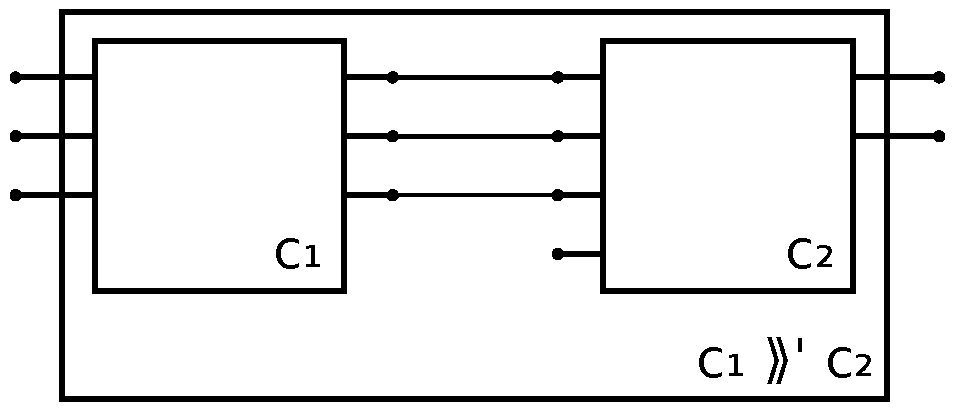
\includegraphics[width=0.6\textwidth]{imgs/sequencing-floating.pdf}}
                        \caption{Example of circuit banned by the type of \AI{\_⟫'\_}.\label{fig:sequencing-floating}}
                    \end{figure}

                \item [No short-circuits] The \AI{Plug} constructor, the only one which can be used for
                    "rewiring" purposes, has a type which forbids connecting multiple sources to the same load.
                    Its argument is a \emph{function from outputs to inputs}.
                    In this way, definitions connecting multiple inputs to the same output are banned,
                    as they are \emph{not} functions from outputs to inputs.
                    Also, when a plug is used between two sub-circuits $c₁$ and $c₂$,
                    a definition in which an \emph{input} of $c₂$ would be left \emph{disconnected} is disallowed by Agda,
                    as such a definition would not be \emph{total}.
                    The diagram on Figure~\ref{fig:plug-seq-disconnected-input} represents such a banned situation:

                    \begin{figure}[h]
                        \centering{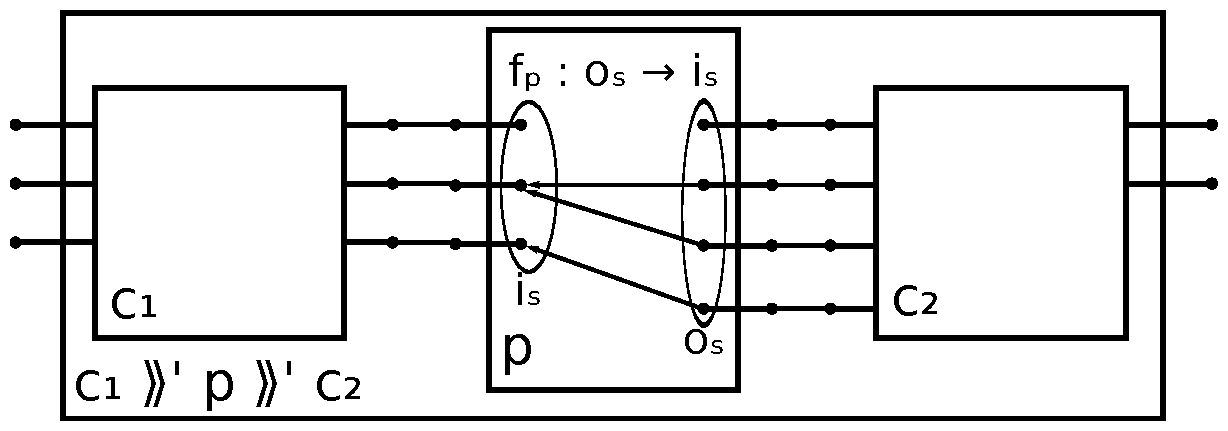
\includegraphics[width=0.9\textwidth]{imgs/plug-seq-disconnected-input.pdf}}
                        \caption{This circuit cannot be constructed because $f_{p}$ is not \emph{total}.\label{fig:plug-seq-disconnected-input}}
                    \end{figure}
            \end{description}

            \subsubsection{Purely combinational vs. possibly sequential}
            \label{subsubsec:comb-vs-seq}
            Circuits in Π-Ware can be \emph{purely combinational} or \emph{sequential}.
            Combinational circuits have no internal state and can be simulated without regarding past inputs.
            A very simple semantics is defined over the circuit datatype in order to distinguish
            these two classes of circuits.

            The semantic function is the \AF{comb'} predicate, defined over low-level (\AF{ℂ'}).
            The \AF{comb'} function returns an Agda \AF{Set} which can be either \AF{⊤}
            (the \AF{Set} with one value) or \AF{⊥} (the \AF{Set} with no values).
            This returned \AD{Set} can therefore be interpreted as a \emph{truth value}.
            Listing~\ref{lst:comb-core} shows the code of the \AF{comb'} predicate

            \begin{listing}[h]
                \ExecuteMetaData[code/agda/latex/PiWare/Circuit/Core.tex]{comb-core-decl}
                \ExecuteMetaData[code/agda/latex/PiWare/Circuit/Core.tex]{comb-core}
                \caption{Predicate telling whether a low-level circuit is purely combinational.\label{lst:comb-core}}
            \end{listing}

            Notice how the fundamental constructors (\AI{Nil}, \AI{Gate} and \AI{Plug}) \emph{always}
            build purely combinational circuits, while \AI{DelayLoop} always produces circuits with internal state.
            The structural constructors (\AI{\_⟫'\_}, \AI{\_|'\_} and \AI{\_|+'\_}) yield a combinational circuit
            \emph{if and only if} \emph{both} of its arguments are themselves combinational.
            This is expressed by using the product type constructor \AF{\_×\_},
            which corresponds to a logical conjunction.

            This categorization of circuits as stateful or stateless has one main goal:
            To avoid the evaluation of \emph{combinational loops}.
            Their presence in a circuit is almost always a design mistake.
            Altera™, for example, explains in their manual of "Recommended Design
            Practices"\footnote{\url{http://www.altera.com/literature/hb/qts/qts\_qii51006.pdf}}:

            \begin{quote}
                Combinational loop behavior generally depends on relative propagation delays
                through the logic involved in the loop. As discussed, propagation delays can change,
                which means the behavior of the loop is unpredictable.
            \end{quote}

            In Π-Ware, the semantics of the \AI{DelayLoop} constructor, and the clear \emph{partitioning}
            of circuits into combinational or sequential done by the \AF{comb'} predicate guarantee that:

            \begin{itemize}
                \item The only way to create a loop in a circuit (\AI{DelayLoop}) also introduces a
                    delay\footnote{in hardware terms, a \emph{clocked latch}.}.

                \item Combinational simulation (ignoring past inputs) only happens when
                    the circuit is provably cycle-free, thus stateless and free of race conditions.
            \end{itemize}


    \section{Abstraction Mechanisms}
    \label{sec:circuit-abstraction}
        Several of the definitions (modules, datatypes, functions) of Π-Ware
        are parameterized in order to improve code reuse.
        The library allows for a choice of the type of data carried in individual wires,
        the types that serve as inputs and outputs to circuits,
        and the set of fundamental gates from which circuits are built.

        In this section we present how this flexibility is achieved,
        and which requirements are imposed upon the parameters in each case of parameterization.
        Furthermore, we discuss the motivation behind the chosen requirements,
        based on the general goals of Π-Ware as well as the wish to impose as few constraints as possible.


        \subsection{Atoms}
        \label{subsec:atoms}
            In \acp{EDSL} of the current Lava family~\cite{observable-sharing-circuits},
            only values of type \mintinline{haskell}{Bool} and \mintinline{haskell}{Int}
            can be carried by the "wires", and circuits can only operate on inputs and outputs
            which are tuples or lists of these basic types.

            There is a little more flexibility in ForSyDe~\cite{forsyde1999},
            where the \mintinline{haskell}{ProcType} type class determines what types can be used
            as input and output types of \emph{process functions} (combinational circuits).
            ForSyDe has predefined instances of \mintinline{haskell}{ProcType} for fixed-width numeric types
            (\mintinline{haskell}{Int8}, \mintinline{haskell}{Int16}, etc.) and \mintinline{haskell}{Bool},
            while relying on \emph{Template Haskell} to generate instances for user-defined \emph{enumeration types}
            at compile time.

            Π-Ware's approach is similar to ForSyDe's, in that it shares the same goal
            (to carry in the wires any type belonging to a type class).
            However, Π-Ware does not use any metaprogramming, and uses dependent types
            to ensure that the provided instances satisfy desired properties.
            The \ARR{Atomic} record (shown in Listing~\ref{lst:atomic})
            captures the requirements for a type to be carried in the wires of a circuit.

            \begin{listing}[h]
                \centering{\ExecuteMetaData[code/agda/latex/PiWare/Atom.tex]{Atomic}}
                \caption{The \AD{Atomic} type class.\label{lst:atomic}}
            \end{listing}

            The fields \AL{Atom} and \AL{|Atom|-1} determine, respectively,
            the Agda \AD{Set} to be used as basis and \emph{how many elements} of this \AD{Set}
            are to be used as atoms (the number of atoms is actually \AF{|Atom|} \AY{=} \AI{suc} \AL{|Atom|-1}).

            Then there are the fields \AL{n→atom} and \AL{atom→n}, which define a \emph{bijection}
            between the \AL{Atom} type and \AD{Fin} \AF{|Atom|} (naturals from \AI{zero} to \AL{|Atom|-1}).
            Finally, the two last fields in \ARR{Atomic} are proofs
            that \AL{n→atom} and \AL{atom→n} are inverses of each other,
            therefore proving that they are also bijections.

            \subsubsection{Instance for \texttt{Bool}}
            \label{subsubsec:atomic-bool}
            Included with Π-Ware there is already a predefined instance of \ARR{Atomic} for \AD{Bool}
            (the boolean type in Agda's standard library).
            Knowing the meaning of each field, the definitions comprising the instance
            are mostly easy to understand.
            First, we start by defining the cardinality of the set of values we are interest in
            (\AD{B} is used as synonym for \AD{Bool}):

            \begin{center}
                \ExecuteMetaData[code/agda/latex/PiWare/Atom/Bool.tex]{cardinality}
            \end{center}

            Now, before defining the bijections that enumerate the set of atoms,
            we give more convenient \emph{names} to the elements of \AD{Fin} \AF{|B|} used in the enumeration
            by using an Agda feature known as \emph{pattern synonyms}:

            \begin{center}
                \ExecuteMetaData[code/agda/latex/PiWare/Atom/Bool.tex]{pattern-synonyms}
            \end{center}

            The usage of the \AI{Absurd\#} pattern becomes clearer when we take a look at
            the definitions of the bijections themselves:

            \begin{center}
                \ExecuteMetaData[code/agda/latex/PiWare/Atom/Bool.tex]{nToBool}
            \end{center}

            In the case of the \AI{Absurd\#} pattern, there is no need to provide a right-hand side
            to the equation, as the Agda typechecker can verify that
            there is no \AB{x} such that \AI{Fs} \AY{(}\AI{Fs} \AB{x}\AY{)} belongs to \AD{Fin} \AN{2}.

            Finally, there are the proofs stating that \AF{n→B} has a two-sided inverse (namely, \AF{B→n}),
            and, therefore, it is a bijection. The proofs use simple case analysis (and reflexivity).

            \begin{center}
                \ExecuteMetaData[code/agda/latex/PiWare/Atom/Bool.tex]{inv-Bool}
            \end{center}

            \subsubsection{Other possibly interesting instances}
            \label{subsubsec:atomic-other}
            Even though currently \AD{Bool} (from the Agda standard library) is the only type for which
            there is already a predefined instance of \ARR{Atomic}, other types could be interestingly used as atoms.
            For example:

            \begin{description}
                \item[Three-valued logic types]
                    Representing the values \texttt{TRUE}, \texttt{FALSE} and \texttt{UNKNOWN}
                \item[IEEE1164 nine-valued logic]
                    Standardized logic used widely in industry as a VHDL/Verilog type.
                    Besides the usual \texttt{FALSE} and \texttt{TRUE} logical values
                    (represented respectively by '0' and '1'),
                    it accommodates also the following others:
                    \begin{itemize}
                        \item \texttt{'Z'}: \emph{High impedance}, means output is not being driven.
                        \item \texttt{'X'}: \emph{Strong drive, unknown logic value}.
                        \item \texttt{'W'}: \emph{Weak drive, unknown logic value}.
                        \item \texttt{'L'}: \emph{Weak drive, logic zero}.
                        \item \texttt{'H'}: \emph{Weak drive, logic one}.
                        \item \texttt{'U'}: \emph{Uninitialized}. Used as default initial value in simulation.
                        \item \texttt{'-'}: \emph{Don't care}.
                    \end{itemize}
                \item[Numeric types]
                    For example, some binary type equivalent to one of Haskell's fixed-size integers
                    (\mintinline{haskell}{Int8}, \mintinline{haskell}{Int16}, etc.).
                    The problem with big \AD{Atom} types, however, is that the enumeration functions
                    using Peano-based finite naturals as indices (\AD{Fin} \AB{n}) can become quite
                    inefficient for very large \AB{n}.
            \end{description}

            For this reason it is recommended to choose a \emph{simple and small} type to use as \AD{Atom},
            and represent the mapping between complex types and a sequence of \AD{Atom}s using
            the \ARR{⇓W⇑} (\texttt{Synthesizable}) type class, detailed in Section~\ref{subsec:synthesizable}.


        \subsection{Gate library}
        \label{subsec:gate-library}
            Besides being parameterized by the type of \AD{Atom}s that can be carried in their wires,
            Π-Ware low-level circuit descriptions (\AD{ℂ'}) are also parameterized by
            a \emph{library of fundamental gates} upon which circuits are built.

            There are several interesting possible gate libraries which could be used to describe circuits,
            among which:

            \acrodef{DSP}{Digital Signal Processing}
            \begin{itemize}
                \item \emph{Functionally complete} sets of boolean functions such as
                    $\{ \text{\texttt{NAND}} \}$, $\{ \text{\texttt{NOR}} \}$ or
                    $\{ \text{\texttt{NOT}}, \text{\texttt{AND}}, \text{\texttt{OR}} \}$
                    (predefined in the Π-Ware library).
                \item Arithmetic primitives over boolean vectors, such as $\{ \text{\texttt{\_+\_}}, \text{\texttt{\_*\_}} \}$.
                \item A logic-arithmetic library together with some purpose-specific primitives,
                    for example cryptographic and \ac{DSP} functions.
            \end{itemize}

            A gate library is defined as an element of the \ARR{Gates} record type, shown in Listing~\ref{lst:gates}.

            \begin{listing}[h]
                \ExecuteMetaData[code/agda/latex/PiWare/Synthesizable.tex]{Word}
                \newline
                \ExecuteMetaData[code/agda/latex/PiWare/Gates.tex]{Gates}
                \caption{Definition of a gate library: the \ARR{Gates} record.\label{lst:gates}}
            \end{listing}

            The first field of the \ARR{Gates} record (\AL{|Gates|}) determines \emph{how many}
            gates the library has, and consequently also the \emph{the type used as gate index}
            (or \emph{gate identifier}), which is \AF{Gates\#} \AY{=} \AF{Fin} \AL{|Gates|}.

            For each gate identifier, the functions \AL{ins} and \AL{outs} determine, respectively,
            the size of the input and output of that gate; therefore together they determine the gate's \emph{interface}.

            Finally, the \AL{spec} field determines the \emph{functional specification} of a given gate identifier.
            Notice how the whole \AM{Gates} module is parameterized by an instance of \ARR{Atomic}.
            In this way, the \AL{spec} function yields, given a gate identifier, a function over \emph{words}
            (\AD{Atom} vectors) of the correct length.
            This functional specification of each fundamental gate is used for the \emph{simulation semantics}.

            \subsubsection{Instance for \texttt{BoolTrio}}
            \label{subsubsec:gates-booltrio}
            One specific instance of gate library is already defined in the Π-Ware library
            (in module \AM{PiWare.Gates.BoolTrio}): the usual set of boolean gates
            $\{ \text{\texttt{NOT}}, \text{\texttt{AND}}, \text{\texttt{OR}} \}$,
            together with the constants $\{ \text{\texttt{FALSE}}, \text{\texttt{TRUE}} \}$.
            The first definitions in that module establish that the library contains five gates:

            \begin{center}
                \ExecuteMetaData[code/agda/latex/PiWare/Gates/BoolTrio.tex]{cardinality}
            \end{center}

            Then, as already done in the instance of \ARR{Atomic}, we define some \emph{pattern synonyms}
            to make the gate identifiers more readable:

            \begin{center}
                \ExecuteMetaData[code/agda/latex/PiWare/Gates/BoolTrio.tex]{pattern-synonyms}
            \end{center}

            The next step is to define the \emph{interface} of each gate in the library.
            All gates have exactly one output, while the number of inputs vary from 0 to 2.

            \begin{center}
                \ExecuteMetaData[code/agda/latex/PiWare/Gates/BoolTrio.tex]{ins-outs}
            \end{center}

            Finally, the last piece of information needed to define the gate library is
            the functional specification of each gate.

            \begin{center}
                \ExecuteMetaData[code/agda/latex/PiWare/Gates/BoolTrio.tex]{spec}
            \end{center}

            Notice that the gates use \AD{Bool} from Agda's standard library as their \AD{Atom} type.
            Also the logic operators from the standard library (\AM{Data.Bool}) are used in the specification.
            With all the necessary pieces of the puzzle in hand, the definition of the \AD{BoolTrio}
            gate library is as follows:

            \begin{center}
                \ExecuteMetaData[code/agda/latex/PiWare/Gates/BoolTrio.tex]{BoolTrio}
            \end{center}

            \subsubsection{Assumed correctness}
            \label{subsubsec:gates-assumed-correctness}
            Later, in Section~\ref{subsec:functional-correctness}, we will give a precise definition
            for what is considered the \emph{functional correctness} of a circuit; its \emph{compliance}
            to a certain functional specification.

            Usually, the proof of functional correctness for a circuit is built using, in some way,
            the correctness proofs of its subcomponents.
            However, fundamental gates have no subcomponents, so their correctness is assumed.
            By definition, the simulation semantics of a fundamental gate is equal to the \AL{spec}
            function given for it in the gate library definition.

            \subsubsection{Relation to synthesis}
            \label{subsubsec:relation-to-synthesis}
            Even though fundamental gates have no subcomponents \emph{at the Π-Ware level},
            they are not in any way directly synthesizable to \ac{VHDL}.
            To convert a Π-Ware circuit to \ac{VHDL}, each fundamental gate in the library being used
            needs to have a corresponding excerpt of \ac{VHDL} code representing it.

            This feature is not integrated in the current version of Π-Ware, but assuming the existence
            of a hierarchy of datatypes representing \ac{VHDL} code, and specifically the existence
            of a type \AD{VHDLEntity}, we could have an extra field in the \ARR{Gates} record, as such:

            \begin{center}
               \AL{netlist} \AY{:} \AY{(}\AB{g} \AY{:} \AD{Fin} \AL{|Gates|}\AY{)} \AY{→} \AD{VHDLEntity} \AY{(}\AL{ins} \AB{g}\AY{)} \AY{(}\AL{out} \AB{g}\AY{)}
            \end{center}

            The \AD{VHDLEntity} is also parameterized by the input and output sizes of the circuit,
            tying the Π-Ware fundamental gate interface with the \ac{VHDL} abstract syntax.



        \subsection{High-level circuit datatype}
        \label{subsec:high-level-circuit}
            When presenting the low-level circuit datatype (\AD{ℂ'}) on Section~\ref{sec:circuit-syntax},
            it was mentioned that the representation using \AD{ℂ'} is untyped and unstructured, i.e.,
            all circuit inputs and outputs at that level are just sequences of \AD{Atom}s (for example, bits).

            However, the user of Π-Ware is not supposed to actually model circuits using the \AD{ℂ'} datatype.
            There is a layer of abstraction sitting on top of \AD{ℂ'},
            and circuits at this higher level have inputs and outputs with Agda types.
            This layer is coded as the \AD{ℂ} datatype, shown in Listing~\ref{lst:Circuit}.

            \begin{listing}[h]
                \centering{\ExecuteMetaData[code/agda/latex/PiWare/Circuit.tex]{Circuit}}
                \caption{High-level circuit datatype (\AD{ℂ}).\label{lst:Circuit}}
            \end{listing}

            In contrast to the low-level (\AD{ℂ'}) circuit type, \AD{ℂ} is parameterized by two \AD{Set}s
            and has only one constructor – \AI{Mkℂ} – which packs the low-level circuit description
            with information on how to convert between the input/output Agda types (resp. \AB{α} and \AB{β})
            and the appropriately-sized \emph{words}\footnote{A \emph{word} is a vector of \AD{Atom}s.}
            used in the low level.
            This conversion information is coded in the two first parameters passed to the \AI{Mkℂ} constructor,
            which are \emph{instances} of the \ARR{⇓W⇑} type class (pronounced \texttt{Synthesizable}),
            This type class is covered in more detail on Section~\ref{subsec:synthesizable}.
            Roughly, it ensures that a type can be converted to \emph{words} (vectors of \AD{Atom}s).

            Furthermore, notice the \emph{lack of a prime symbol in the name of the datatype}.
            This is a general naming convention:
            whenever there are two versions of a definition, one at a low level of abstraction and one higher,
            the low-level gets the same name of the high-level one, with a prime symbol as suffix.

            The \AM{PiWare.Circuit} module defines also \emph{smart constructors} for \AD{ℂ},
            corresponding to each of the constructors at the low level.
            One example is parallel composition – shown here without passing instance arguments for brevity:

            \begin{center}
                \ExecuteMetaData[code/agda/latex/PiWare/Circuit.tex]{par}
            \end{center}

            Using a \emph{gate library} together with these smart constructors, one can model
            hardware circuits operating over Agda types.
            One very simple example is a \texttt{XOR} circuit (shown in Listing~\ref{lst:xor-sample}),
            built using the \texttt{BoolTrio} gate library mentioned before.
            The block diagram in Figure~\ref{fig:xor-sample} illustrates the architecture of such circuit.

            \begin{figure}[h]
                \centering{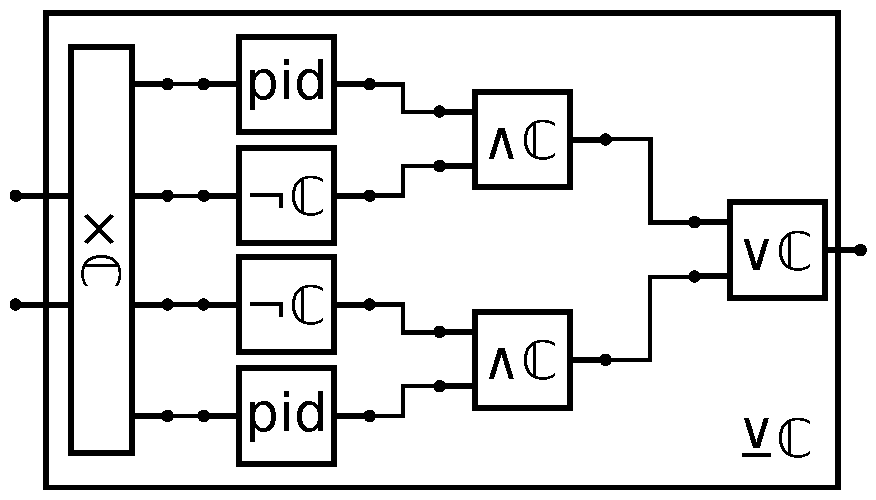
\includegraphics[width=0.50\textwidth]{imgs/xor-sample.pdf}}
                \caption{Architecture of a sample \texttt{XOR} gate.\label{fig:xor-sample}}
            \end{figure}

            \begin{listing}[h]
                \centering{\ExecuteMetaData[code/agda/latex/PiWare/Samples/BoolTrioComb.tex]{fundamentals}}
                \newline
                \centering{\ExecuteMetaData[code/agda/latex/PiWare/Samples/BoolTrioComb.tex]{xor}}
                \caption{Example of a \texttt{XOR} gate built with the \texttt{BoolTrio} library.\label{lst:xor-sample}}
            \end{listing}

            Again in this example, as customary, we renamed \AD{Bool} to \AD{B},
            and \AF{pid} is the \emph{identity plug}.
            The identity plug can be substituted in the netlist by a \emph{bus} (with the adequate size),
            and is defined (together with other useful plugs) in the \AM{PiWare.Plugs} module.


        \subsection{The \texttt{Synthesizable} type class}
        \label{subsec:synthesizable}
            The "connection" between the low-level (\AD{ℂ'}) and high-level (\AD{ℂ}) circuit types
            is done by the \ARR{⇓W⇑} type class (pronounced \texttt{Synthesizable}).
            Instances of the \ARR{⇓W⇑} class define a mapping between a given Agda type
            and an appropriately-sized \emph{word} type.
            Word types (\AD{W} \AB{n}, for some \AB{n}) are \emph{synthesizable} to \ac{VHDL} vectors,
            thus the name of the class.
            Listing~\ref{lst:Synth} shows the definition of \ARR{⇓W⇑}:

            \begin{listing}[h]
                \ExecuteMetaData[code/agda/latex/PiWare/Synthesizable.tex]{Word}
                \newline
                \ExecuteMetaData[code/agda/latex/PiWare/Synthesizable.tex]{Synth}
                \caption{The \ARR{⇓W⇑} (Synthesizable) type class.\label{lst:Synth}}
            \end{listing}

            The type class has two parameters: the type which it encodes (\AB{α}),
            and the size of the \emph{word type} to which \AB{α} corresponds (\AB{i}).
            Notice that the size parameter is passed \emph{implicitly}, because in some occasions
            Agda might be able to automatically infer (by unification) this value.

            One can imagine that all \emph{finite types} (types with finitely many elements)
            can be made synthesizable under the definition of \ARR{⇓W⇑}, given a certain encoding scheme.
            Intuitively, any finite type is isomorphic to Agda's \AD{Fin} \AB{n}, for some \AB{n},
            for which an instance of \ARR{⇓W⇑} can easily be defined.

            We do not give a proof of this statement, but one way of doing it would be to translate
            Agda datatype definitions into a sum-of-products view and then use a standardized
            encoding scheme (for example, some form of \emph{Church encoding}).

            Π-Ware does \emph{not} provide facilities for mapping arbitrary Agda datatypes into
            a sum-of-products view (we believe this is the domain of a \emph{generic programming} library,
            not of a hardware \ac{EDSL}).
            However, Π-Ware \emph{does} provide predefined instances of \ARR{⇓W⇑} for units (\AD{⊤}),
            booleans (\AD{Bool}), products (\AD{\_×\_}), vectors (\AD{Vec}) and sums (\AD{\_⊎\_}),
            in order to facilitate working with complex types when modelling hardware.

            One interesting instance to look at is the one for Agda's standard library vectors (\AD{Vec}),
            shown in Listing~\ref{lst:Synth-Vec}.

            \begin{listing}[h]
                \centering{\ExecuteMetaData[code/agda/latex/PiWare/Synthesizable.tex]{Synth-Vec}}
                \caption{Predefined instance of \ARR{⇓W⇑} for fixed-length vectors.\label{lst:Synth-Vec}}
            \end{listing}

            In the \AF{down} definition,
            the \emph{bind} (\AF{>>=}) operator is defined as \AF{concat} \AO{∘} \AF{map}, i.e.,
            first each element of the vector is serialized (using the passed instance for \AB{α}),
            then all the words (each with size \AB{i}) are concatenated, giving a total size of
            \AY{(}\AB{n} \AF{*} \AB{i}\AY{)}.

            To convert a serialized \AD{Vec} back \AF{up}, first the given word is \AF{group}ed
            into \AB{n} smaller words (each of size \AB{i}), which is possible because the size of
            the passed word is \AY{(}\AB{n} \AF{*} \AB{i}\AY{)}.
            Then, ignoring the proof object returned by \AF{group} (which is in the second position
            of a pair, therefore we take \AL{proj₁}), we map the \AF{up} instance of \AB{α} over
            each of the smaller words, obtaining in this way an element of type
            \AD{Vec} \AB{α} \AB{n}.

            \subsubsection{Proof of bijection}
            \label{subsubsec:proof-bijection}
            It is very desirable that the pair of methods in \ARR{⇓W⇑} – \AL{⇓} (\texttt{down}) and
            \AL{⇑} (\texttt{up}) – are defined as inverses of each other, that is:

            \begin{center}
                \AY{∀} \AY{(}\AB{x} \AY{:} \AB{α}\AY{)} \AY{→} \AL{⇑} \AY{(}\AL{⇓} \AB{x}\AY{)} \AF{≡} \AB{x}
                \\
                \AY{∀} \AY{(}\AB{w} \AY{:} \AD{W} \AB{i}\AY{)} \AY{→} \AL{⇓} \AY{(}\AL{⇑} \AB{w}\AY{)} \AF{≡} \AB{w}
            \end{center}

            With this property, the correctness of a low-level circuit (\AD{ℂ'}) translates trivially
            via \AL{⇓} and \AL{⇑} to the correctness of it's high-level correspondent.

            We considered including the proof that \AL{⇓} and \AL{⇑} also as methods of the \ARR{⇓W⇑} class,
            thereby \emph{requiring} the user to prove this property before using any high-level type with Π-Ware.
            Ultimately, given the experience we had in writing these proofs for some of the \ARR{⇓W⇑} instances predefined
            in Π-Ware, we decided against inclusion as required methods.
            This would be too big of an initial burden put on a designer, who would have to prove bijection
            \emph{even before} being able to write any prototype circuit using the intended types.

            \subsubsection{\texttt{Synthesizable} instance for sums}
            \label{subsubsec:synthesizable-sums}
            The instance of \ARR{⇓W⇑} for sums (disjoint unions) is the most complex among all predefined
            instances included with Π-Ware.
            This complexity comes mostly from the need to \emph{distinguish} which set is concerned
            when converting a word "up" (\AL{⇑}).
            Assuming that we want \AL{⇓} and \AL{⇑} to form a bijection (no information may be lost),
            let's first calculate how many atoms are necessary to represent a sum.

            With a given encoding for set \AB{α} (\AB{sα} \AY{:} \ARR{⇓W⇑} \AB{α} \AY{\{}\AB{i}\AY{\}})
            and one for β (\AB{sβ} \AY{:} \ARR{⇓W⇑} \AB{β} \AY{\{}\AB{j}\AY{\}}),
            it is clear that at least \AB{i} \AF{⊔} \AB{j} atoms are necessary to encode \AB{α} \AD{⊎} \AB{β};
            the size of a sum is at least the maximum among the sizes of its summands.
            Furthermore, it is necessary to somehow encode the choice (whether the sum was built from
            the left (\AL{inj₁}) or the right (\AL{inj₂}). This requires at least one more atom,
            bringing the size to \AI{suc} \AY{(}\AB{i} \AF{⊔} \AB{j}\AY{)}.

            The predefined instance for sums included with Π-Ware is shown on Listing~\ref{lst:Synth-Sum}.

            \begin{listing}[h]
                \centering{\ExecuteMetaData[code/agda/latex/PiWare/Synthesizable.tex]{Synth-Sum}}
                \caption{Predefined instance of \ARR{⇓W⇑} for sums.\label{lst:Synth-Sum}}
            \end{listing}

            Besides the encodings of the summands (named \AB{sα} and \AB{sβ},
            given as \emph{instance arguments}), this instance is also passed some extra parameters:
            three \emph{atom indices} (\AB{n}, \AB{m} and \AB{p}) and a proof that \AB{n} and \AB{m} are different.
            The atom index \AB{n} indicates the \AD{Atom} to be used in case the sum is built from the left (\AL{inj₁}).
            and \AB{m} for the case when it is built from the right (\AL{inj₂}).
            They need to be different in order for the choice information not to be lost when synthesizing a sum type.
            At last, the \AB{p} parameter identifies the atom used for padding.

            In the \AF{down} function, the \AF{[\_,\_]} sum \emph{destructor} is used,
            and is passed two functions: one to operate at the left case and one at the right.
            They prepend to the output word an atom identified by either \AB{n} or \AB{m} and pad
            either \AB{a} or \AB{b} to fit \AB{i} \AF{⊔} \AB{j}.

            In the \AF{up} conversion, first the \emph{tag} is used to transform the input word into
            a sum of words (\AD{W} \AB{i} \AD{⊎} \AD{W} \AB{j}),
            then the \AF{map⊎} function is used to apply either the \AL{⇑} instance for \AB{α} or for \AB{β},
            giving the desired result type of \AB{α} \AD{⊎} \AB{β}.

            \subsubsection{Recursive instance search}
            \label{subsubsec:recursive-instance-search}
            To model synthesizable datatypes, we used the Agda way of implementing Haskell's type classes,
            namely, to code a type class as a record type, in which each field corresponds to a method.
            In this analogy, instances are just elements of the record type, and class constraints are
            coded in Agda by passing \emph{instance arguments}~\cite{typeclasses-agda} to the constrained function.
            Arguments passed in this way will be searched among the identifiers available in scope,
            in a type-directed fashion, similar to how the mechanism of instance search works in Haskell.

            However, there was (until recently) a big drawback to Agda's instance search implementation:
            it was not recursive.
            There were some arguments for this decision in the original paper,
            most notably that having fully recursive instance resolution would
            "expose an additional computational model" and that the instance search mechanism
            would need to "perform a reasonably powerful automated proof search".

            During the last years, since the publication of the paper on instance arguments~\cite{typeclasses-agda},
            demand has grown for recursive instance search in Agda, and in a recent contribution to the Agda codebase
            by Guillaume Brunerie\footnote{\url{https://github.com/agda/agda/commit/7ca60fd60aec1b73d9f14aaa6e1aeef184bcca79}},
            costs and benefits were again weighted, and a reasonably efficient implementation was released
            in Agda version 2.4.0.2 (current version at the time of writing this report).

            The impact of this change for Π-Ware is immense.
            Recursive instance resolution removes the need for a great deal of boilerplate code.
            For example, before the advent of recursive resolution, modelling the \texttt{XOR} circuit
            on Listing~\ref{lst:xor-sample} required the user to manually construct instances of \ARR{⇓W⇑}
            for more than 5 types
            ( \AD{𝔹} \AD{×} \AD{𝔹}
            , \AY{(}\AD{𝔹} \AD{×} \AD{𝔹}\AY{)} \AD{×} \AD{𝔹}
            , \AD{𝔹} \AD{×} \AY{(}\AD{𝔹} \AD{×} \AD{𝔹}\AY{)}
            , \AY{(}\AD{𝔹} \AD{×} \AY{(}\AD{𝔹} \AD{×} \AD{𝔹}\AY{)}\AY{)} \AD{×} \AY{(}\AD{𝔹} \AD{×} \AD{𝔹}\AY{)}
            , etc.).
            Now all of this work is done by Agda itself.
            On the other hand, the typechecking time grew a little,
            and this could be a problem when modelling big circuits,
            as discussed in Section~\ref{subsec:current-limitations}.


    \section{Circuit Semantics}
    \label{sec:circuit-semantics}
        In this chapter we will expose and discuss the \emph{semantics} of circuits described using Π-Ware.
        Π-Ware circuits can currently be interpreted in two ways:
        they can be \emph{simulated} (fed with certain inputs and calculate the corresponding outputs)
        or \emph{synthesized} (converted to a \emph{netlist}).
        However, due to the fact the a \emph{deep embedding} is used, other semantics can implemented
        with relative ease, such as timing analysis, power estimation, etc.

        When presenting the simulation semantics, we will separately discuss the simulation of
        purely combinational circuits and of sequential ones,
        also recapitulating the need to distinguish between the two.

        \subsection{Synthesis semantics}
        \label{subsec:synthesis-semantics}
            The synthesis semantics establishes how Π-Ware circuits can be converted to netlists.
            Each element of the low-level circuit datatype (\AD{ℂ'}) has a corresponding netlist
            according to the semantics,
            and to each circuit constructor corresponds a netlist transformation.

            Figure~\ref{fig:semantics-syn-fundamental} shows the semantic rules for the
            fundamental constructors of \AD{ℂ'}, as well as for \AI{DelayLoop}.
            To the left of each diagram there is a typing rule for that case,
            with the constructor's arguments (and their types) above the bar and the result type below it.

            %% TODO: two-column one-page diagram

            \begin{figure}[h]
                \centering{\includegraphics[width=0.93\textwidth]{imgs/semantics-syn-fundamental.pdf}}
                \caption{Synthesis semantics of the fundamental circuit constructors.\label{fig:semantics-syn-fundamental}}
            \end{figure}

            In the diagrams, all ellipses denote elements of type \AD{ℂ'}, i.e., low-level circuits.
            Assuming the existence of a hierarchy of datatypes for representing \ac{VHDL} code
            (as already mentioned in Section~\ref{subsubsec:relation-to-synthesis}),
            each of these ellipses correspond to a \ac{VHDL} \emph{entity} (an element of \AD{VHDLEntity}).

            The line segments connecting the ellipses are signals (\AD{VHDLSignal}) – with their size
            denoted by the variable above the perpendicular "dash" in the segment.
            Each of the little dots on the extremity of a line segment correspond to a \emph{port declaration}
            (\AD{VHDLPortDecl}). The arrows on the line segments indicate the direction of the flow of information.

            \acrodef{FPGA}{Field-Programmable Gate Array}
            It is important that these diagrams \emph{do not prescribe any placement} for the circuit components.
            They denote only \emph{netlists}, i.e., directed graphs in which the nodes are elements of \AD{ℂ'}
            and the edges are the signals connecting them (labeled by signal \emph{size}).
            The actual \emph{placement} of this netlist into physical slots (of an \ac{FPGA} or \ac{ASIC}),
            with the accompanying \emph{routing} of wires, is a further step in the implementation chain,
            \emph{not performed by Π-Ware}.

            The semantics of structural circuit constructors (sequential, parallel, sum) is
            shown in Figure~\ref{fig:semantics-syn-structural}.

            \begin{figure}[h]
                \centering{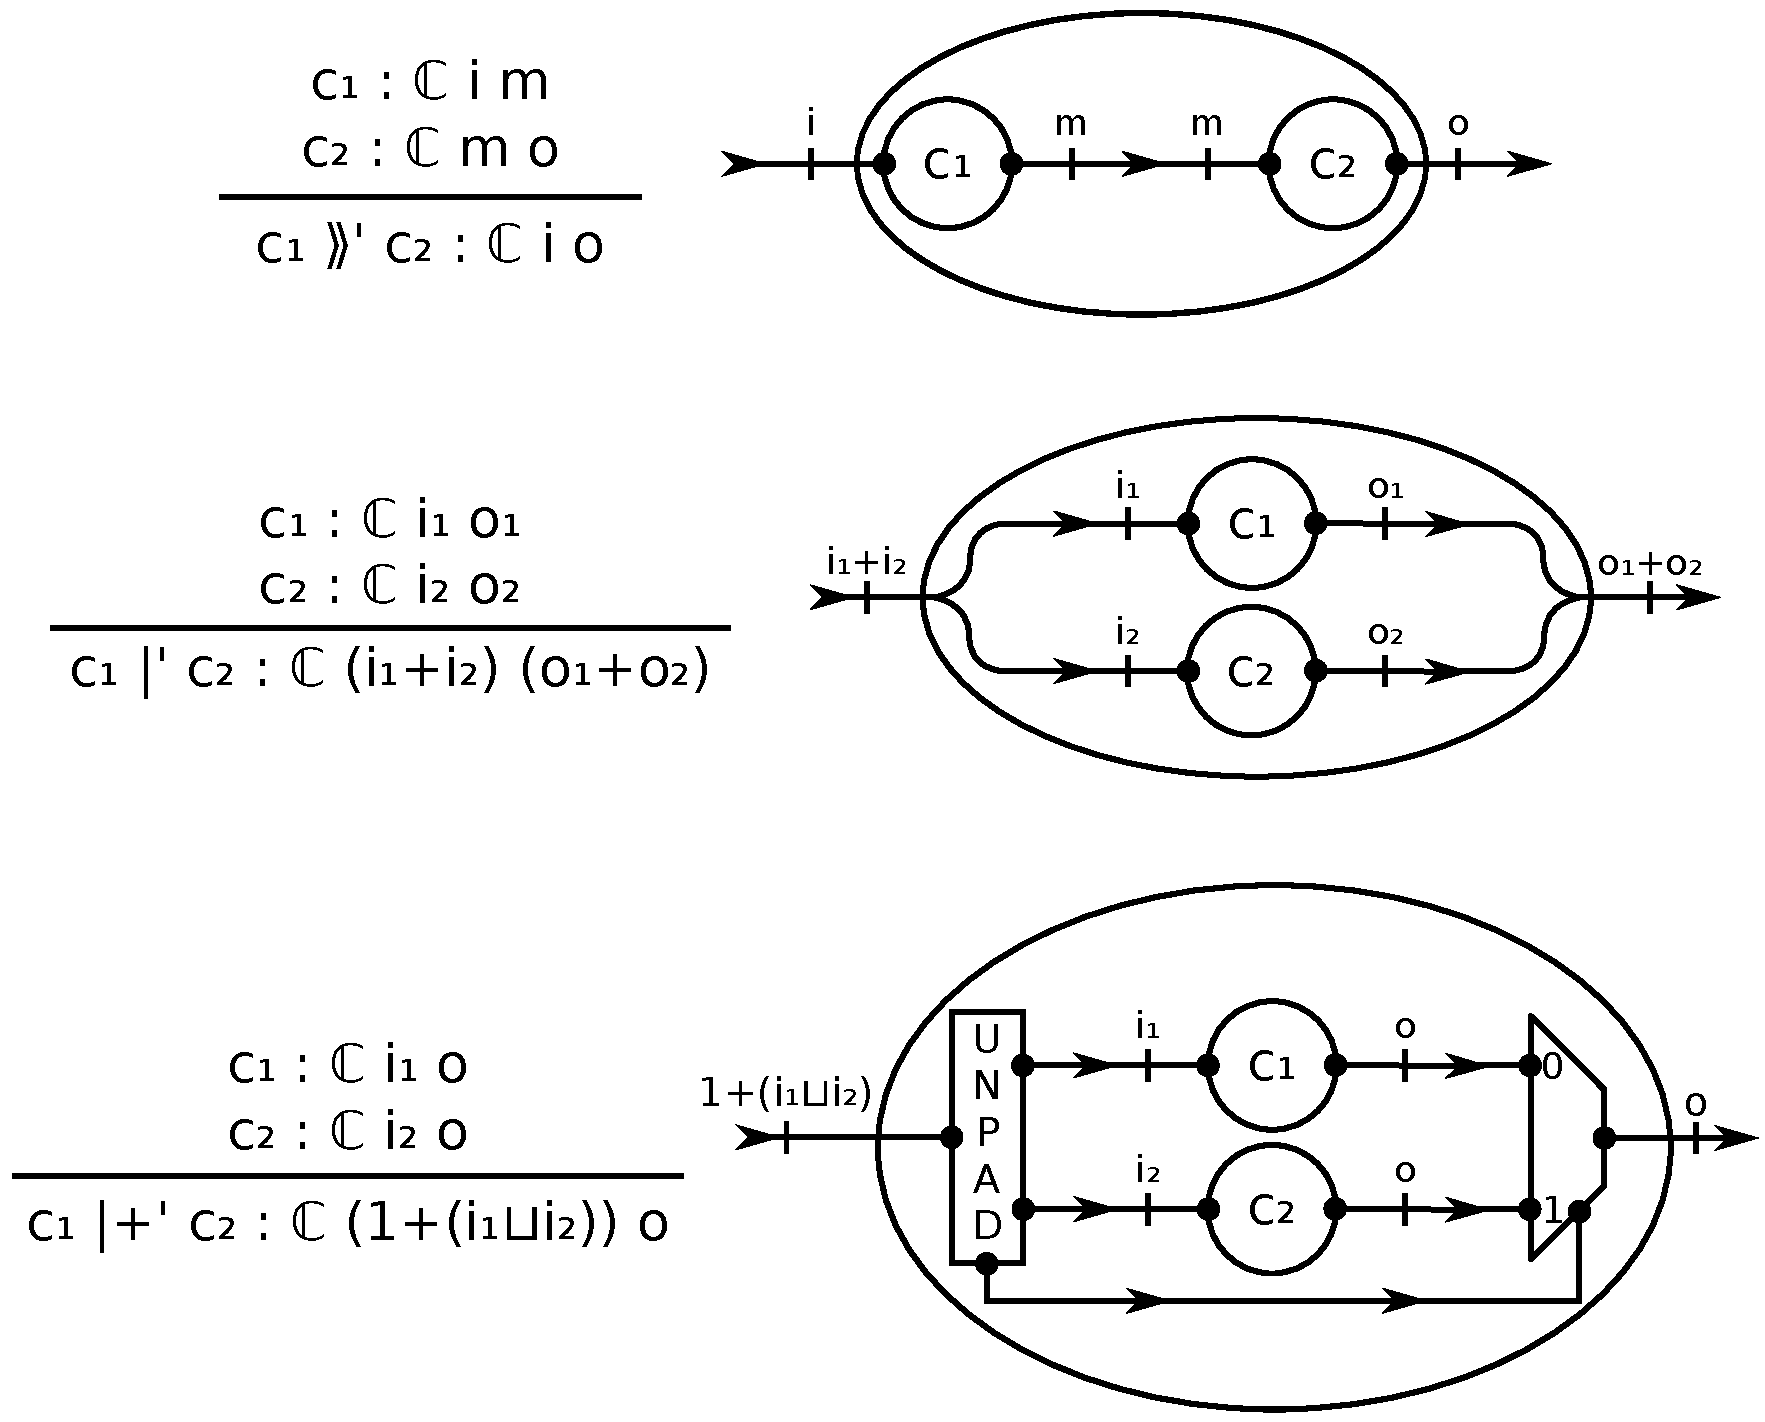
\includegraphics[width=0.93\textwidth]{imgs/semantics-syn-structural.pdf}}
                \caption{Synthesis semantics of structural circuit constructors.\label{fig:semantics-syn-structural}}
            \end{figure}

            In the sum case (\AI{\_|+'\_}), the \texttt{UNPAD} block only "slices" the input into three outputs:
            the tag (first bit) is used as the selector for the \emph{multiplexer}, and the other two outputs
            have, respectively, the first \AB{i₁} and \AB{i₂} bits of the input.
            The diagram on Figure~\ref{fig:semantics-syn-unpad} shows which slices of input go to each
            output of the \texttt{UNPAD} block in the sum case.

            \begin{figure}[h]
                \centering{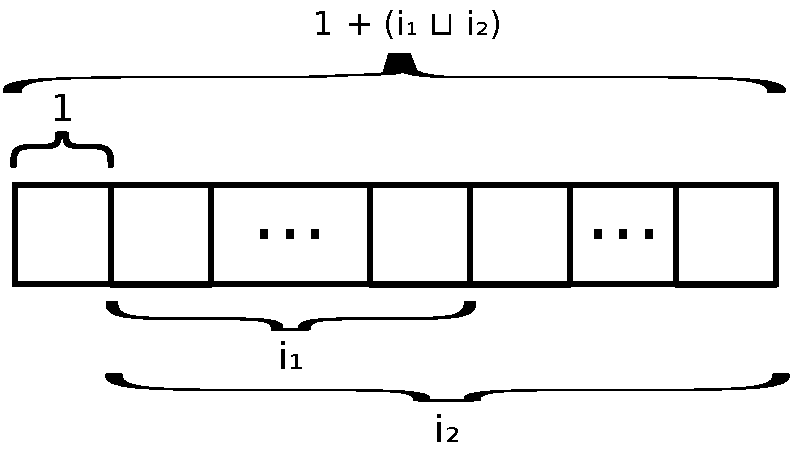
\includegraphics[width=0.60\textwidth]{imgs/semantics-syn-unpad.pdf}}
                \caption{How \texttt{UNPAD} "slices" its input into three outputs.\label{fig:semantics-syn-unpad}}
            \end{figure}

            Finally, it is important to emphasize that the labels \texttt{'0'} and \texttt{'1'}
            were used in the multiplexer only as a mnemonic device.
            The same remark applies to describing the information on the wires as "bits".
            In reality, any \ARR{Atomic} type can flow through the wires, and any two \AD{Atom}s
            can label the inputs of the multiplexer (passed to \AI{\_|+'\_}).


        \subsection{Combinational simulation}
        \label{subsec:combinational-eval}
            As already mentioned in Section~\ref{sec:circuit-syntax},
            the \AF{comb'} predicate determines whether its circuit argument is \emph{purely combinational}.
            In fact, \AF{comb'} can be seen as one (very simple) semantics of circuits (\AD{ℂ'}).
            To recapitulate, here is the type of \AF{comb'}:

            \begin{center}
                \ExecuteMetaData[code/agda/latex/PiWare/Circuit/Core.tex]{comb-core-decl}
            \end{center}

            This predicate is used in several places in the Π-Ware library, particularly in what concerns
            the \emph{simulation} semantics.
            Purely combinational circuits have no notion of time or state, so their simulation semantics
            is modelled as just a function over \emph{words} (\AD{Atom} vectors).

            The Agda function giving a time-independent (combinational) semantics for circuits requires that
            \emph{an element of type \AF{comb'} \AB{c}} be passed as implicit argument – corresponding
            to a proof that circuit \AB{c} is purely combinational.
            Furthermore, this semantics depends on the \emph{gate library} and the
            \AD{Atom} type being used, which are parameters to the \AM{PiWare.Simulation.Core} module as a whole.
            Listing~\ref{lst:eval-core} shows the Agda code for the combinational simulation semantics:

            \begin{listing}[h]
                \centering{\ExecuteMetaData[code/agda/latex/PiWare/Simulation/Core.tex]{eval-core}}
                \caption{Agda code for the combinational simulation semantics of \AD{ℂ'}.\label{lst:eval-core}}
            \end{listing}

            First of all, notice the prime symbol on the function's name (\AF{⟦\_⟧'}),
            indicating that it concerns \emph{low-level} circuits (\AD{ℂ'}).
            From the cases for fundamental constructors, we highlight the usage of the \AF{spec}
            function from the chosen gate library, returning the specification function for a given gate.
            Furthermore, the \AI{DelayLoop} case can be \emph{discharged}, i.e.,
            it is not necessary to provide a definition in this case,
            as \AF{comb'} \AY{(}\AI{DelayLoop} \AB{c}\AY{)} evaluates to \AD{⊥}
            and – by definition – no elements of this type can be constructed.

            The cases for structural constructors are somewhat straightforward.
            Sequencing (\AI{\_⟫'\_}) is interpreted just as function composition.
            In the parallel composition (\AI{\_|'\_}) case, first the input vector is \emph{splitted}, creating a pair.
            Then the \AF{map} function over pairs is used, to apply (respectively) the semantics of \AB{c₁}
            and \AB{c₂} over each element of the pair.
            Finally, both transformed pair elements are concatenated to build the output.
            In the sum (\AI{\_|+'\_}) case, the \AF{untag} function uses the first atom of the input
            to decode it into a sum.
            Then the sum destructor (\AF{[\_,\_]'}) is used with the appropriate functions
            (semantics of \AB{c₁} and \AB{c₂}) to build the output accordingly.

            Notice how the (implicit) arguments of type \AF{comb'} \AB{c} are matched against and passed.
            In the cases for structural constructors, we know that – by definition – the
            \emph{whole circuit is combinational if and only if all its subcircuits are combinational}.
            Therefore, we can pattern match with the \emph{pair constructor} (\AB{p₁} \AI{,} \AB{p₂}),
            and pass each of \AB{p₁} and \AB{p₂} to the calls of \AF{⟦\_⟧'} on the subcircuits.


            \subsubsection{High-level combinational simulation}
            \label{subsubsec:high-sim-comb}
            Analogous to the dichotomy between low-level \emph{circuits} (\AD{ℂ'}) and high-level ones (\AD{ℂ}),
            there are also both low and high-level simulation
            semantics\footnote{There is no such "high-level" concept for the \emph{synthesis} semantics,
                as it concerns actual hardware.}.

            While the low-level simulation semantics (\AF{⟦\_⟧'}) maps a low-level circuit (\AD{ℂ'})
            to a function over \emph{words},
            the high-level simulation semantics (\AF{⟦\_⟧} – shown in Listing~\ref{lst:eval})
            maps a high-level circuit (\AD{ℂ}) to a function over arbitrary (synthesizable) Agda types.

            \begin{listing}[h]
                \centering{\ExecuteMetaData[code/agda/latex/PiWare/Simulation.tex]{eval}}
                \caption{Simulation semantics for high-level circuits (\AD{ℂ}).\label{lst:eval}}
            \end{listing}


        \subsection{Sequential simulation}
        \label{subsec:sequential-eval}
            So-called \emph{sequential} circuits have an internal state,
            and their behaviour is \emph{history-dependent}:
            The current value of a circuit's output depends not only on the current input,
            but also on the history of previous inputs.
            Therefore, to simulate these circuits, there is the need of some concept of \emph{time dimension}
            where the values of inputs and outputs are situated.

            Π-Ware supports modelling and simulating a specific class of sequential circuits,
            namely \emph{synchronous} sequential circuits.
            In synchronous sequential circuits, state transitions in all memory elements happen
            at the same time, and they can only happen at the (rising or falling) \emph{edge}
            of a global clock circuit.
            Because of this \emph{discrete} nature of signals in synchronous circuits,
            they are usually modelled as \emph{streams} in hardware \acp{DSL}.
            This is also the way in which sequential simulation works in Π-Ware:
            it converts a circuit into a function over streams.

            Listing~\ref{lst:eval-seq-core-decl} shows the type of the semantic function for
            sequential simulation of low-level (\AD{ℂ'}) circuits:

            \begin{listing}[h]
                \centering{\ExecuteMetaData[code/agda/latex/PiWare/Simulation/Core.tex]{eval-seq-core-decl}}
                \caption{Type signature of the semantic function for low-level sequential simulation.
                    \label{lst:eval-seq-core-decl}}
            \end{listing}

            This type signature differs from the purely combinational case (depicted in Listing~\ref{lst:eval-core})
            in only two important ways:

            \begin{itemize}
                \item There is no argument of type \AF{comb'} \AB{c} anymore
                    requiring the circuit to be purely combinational.
                \item The result of evaluating the circuit is now "lifted" to the \AD{Stream} setting,
                    that is, it becomes
                    \AD{Stream} \AY{(}\AD{W} \AB{i}\AY{)} \AY{→} \AD{Stream} \AY{(}\AD{W} \AB{o}\AY{)}.
                    instead of \AD{W} \AB{i} \AY{→} \AD{W} \AB{o}.
            \end{itemize}

            The implementation of the history-dependent behaviour needed in sequential simulation
            uses so-called \emph{causal streams}~\cite{essence-dataflow-programming}.
            Even though the type
            \AD{Stream} \AY{(}\AD{W} \AB{i}\AY{)} \AY{→} \AD{Stream} \AY{(}\AD{W} \AB{o}\AY{)}
            is convenient as an \emph{interface} to interact with sequential circuits, it does not
            reflect accurately the way in which synchronous sequential circuits actually work.

            The type of a general stream function (\AD{Stream} \AB{α} \AY{→} \AD{Stream} \AB{β})
            can be read as:

            \begin{quote}
                Given an infinite sequence of values of type \AB{α},
                produce an infinite sequence of values of type \AB{β}.
            \end{quote}

            As such, a general stream function has no notion of \emph{current} value, neither of past,
            and it \emph{can} "look ahead", that is, use future input values to calculate the next output value.
            One example of such a future-anticipating behaviour can be found in the \AF{tail} function
            located in the \AM{Data.Stream} module:

            \begin{center}
                \ExecuteMetaData[code/agda/latex/Report/ChapterPiWare.tex]{stream-tail}
            \end{center}

            This behaviour cannot be realized as a hardware circuit, as it would imply that the
            circuit outputs in clock cycle $t$ the contents of its input in clock cycle $t+1$.


            \subsubsection{Causal step semantics}
            \label{subsubsec:causal-step-semantics}
            Therefore, in Π-Ware, the \emph{sequential semantics} for circuits (\AF{⟦\_⟧*'}) uses a
            helper definition, a so-called \emph{causal step} semantics.
            A \emph{causal step function} is a function which, given a \emph{causal context},
            produces \emph{one} next value of the output stream.
            Listing~\ref{lst:causal-types} shows the types used in Π-Ware to represent these concepts.

            \begin{listing}[h]
                \centering{\ExecuteMetaData[code/agda/latex/Data/CausalStream.tex]{causal-context}}
                \newline
                \centering{\ExecuteMetaData[code/agda/latex/Data/CausalStream.tex]{causal-step}}
                \caption{Types used to model causal streams.\label{lst:causal-types}}
            \end{listing}

            A \emph{causal context} with values of type \AB{α} is written as \AD{Γc} \AB{α}.
            It is implemented as a \emph{type synonym} of Agda's non-empty lists.
            In this way, there is always a current value (head), while the past (tail) might be empty.
            In some places, when pattern matching non-empty lists, a comma (\AI{\_,\_}) is used
            instead of the normal \emph{cons} operator (\AI{\_∷\_}), to avoid confusion with general lists.

            The \emph{causal step semantics} (\AF{⟦\_⟧c}) maps a circuit into a \emph{causal step function},
            i.e., given a circuit, it returns the function which has current and past inputs as arguments
            and produces the immediately next output as result.
            The code for \AF{⟦\_⟧c} is shown in Listing~\ref{lst:eval-causal}.

            \begin{listing}[h]
                \centering{\ExecuteMetaData[code/agda/latex/PiWare/Simulation/Core.tex]{eval-causal}}
                \caption{Causal step semantics for sequential circuits.\label{lst:eval-causal}}
            \end{listing}

            In the \AI{Nil}, \AI{Gate} and \AI{Plug} cases, the purely combinational semantic function
            is called (ignoring past inputs), passing (implicitly) the necessary proof of purity.
            In the definition of \AF{⟦\_⟧c} for \AI{\_⟫'\_}, the context of \AB{c₁} is just the context
            of the sequence block as a whole, while the context of \AB{c₂} consists of the \emph{outputs}
            of \AB{c₁}.
            These outputs are calculated by \emph{mapping} the causal step function (\AF{⟦\_⟧c})
            over \emph{all previous} contexts of \AB{c₁} (from most recent to oldest, given by \AF{tails⁺}).

            The parallel composition (\AI{\_|'\_}) case has the expected definition:
            it splits the input context pointwise at offset \AB{i₁},
            then applies \AF{⟦} \AB{c₁} \AF{⟧c} and \AF{⟦} \AB{c₂} \AF{⟧c} correspondingly and concatenates the results.
            In the sum (\AI{\_|+'\_}) case, the past part of the context is seggregated into a product
            with only \emph{left summands} in the first projection and \emph{right summands} in the second.
            The type of \AF{untagList} helps to clarify its purpose:

            \begin{center}
                \ExecuteMetaData[code/agda/latex/PiWare/Synthesizable.tex]{untagList-decl}
            \end{center}

            These two seggregated pasts are then passed as the pasts of \AB{c₁} and \AB{c₂}, respectively.
            The definition of \AI{\_|+'\_} is completed by pattern matching on the sum generated
            by \AF{untag} \AY{\{}\AB{i₁}\AY{\}} \AB{w₀}, which gives the current input
            (\AB{w⁰₁} resp. \AB{w⁰₂}) to be passed in the recursive calls with the subcircuits
            (\AF{⟦} \AB{c₁} \AF{⟧c} resp. \AF{⟦} \AB{c₂} \AF{⟧c}).

            It is important to note that, had we used a naïve stream semantics for sequential circuits,
            it would not be possible to define \AF{untagList}.
            Given a stream of sums, we \emph{cannot} produce a product of streams in which each component
            has only \emph{left summands} or \emph{right summands}.
            Using a naïve stream semantics, the function to seggregate the input stream would need to have
            the following type:

            \begin{center}
                \ExecuteMetaData[code/agda/latex/Report/ChapterPiWare.tex]{seggregateStream-decl}
            \end{center}

            If, for example, the input stream contains no left summand whatsoever, then
            no element is available to build the first component of the
            pair – a \emph{stream of lefts} – therefore there is no total definition for \AF{seggregateSums}.
            On the other hand, if we substitute an infinite input stream for a causal context then
            the "seggregation" becomes easy: in case the input context
            contains no left summand, the first element of the product is simply an empty context.


            \AI{DelayLoop} is the most important case of \AF{⟦\_⟧c}, and a bit more involved.
            It calls a helper function (\AF{delay})
            expressing the behaviour of the memory element \emph{inside} the \AI{DelayLoop} block
            (as depicted in Figure~\ref{fig:semantics-syn-fundamental}).
            Listing~\ref{lst:delay} shows the definition of \AF{delay}.

            \begin{listing}[h]
                \raggedleft{\ExecuteMetaData[code/agda/latex/PiWare/Simulation/Core.tex]{delay}}
                \caption{Function expressing the behaviour of a circuit memory element.\label{lst:delay}}
            \end{listing}

            It consists of just "uncurrying" another local definition (\AF{delay'}) which actually
            performs the work.
            This indirect definition is necessary to pass Agda's \emph{termination checker},
            which requires recursive calls to be performed on at least one \emph{structurally smaller}
            argument – in this case, the list of past inputs (\AB{w⁻¹} \AI{∷} \AB{w⁻} becomes \AB{w⁻¹}).

            The \AB{c} parameter to \AF{delay} is the \emph{combinational} subcircuit inside the \AI{DelayLoop} block,
            thus its type (\AB{c} \AY{:} \AY{(}\AB{i} \AF{+} \AB{l}\AY{)} \AY{(}\AB{o} \AF{+} \AB{l}\AY{)})
            includes the amount of wires (\AB{l}) "looping back" through the memory element.
            In the base case (empty past), \AF{delay'} simulates \AF{⟦} \AB{c} \AF{⟧'}
            with an \emph{undefined} state – consisting of \AD{Atom}s indexed by zero (\AI{Fz}).
            In the recursive case, the state is calculate by a recursive call,
            where the "current" input has been substituted by the first past value (\AB{w⁻¹}) and the "past"
            by the even farther past (\AB{w⁻}).

            The current implementation of \AF{delay} is quite inefficient, as the recursive call calculates
            the same values several times; a problem similar to what happens in a naïve recursive
            implementation of the Fibonacci sequence.
            As in the Fibonacci case, \emph{memoization} techniques could also be used to
            improve the performance of \AF{delay}.

            \subsubsection{From step function to stream function}
            \label{subsubsec:step-stream}
            The \emph{causal step function} (\AF{⟦\_⟧'}) produces only the next value of the
            output stream, but the desired interface for simulation is one which, given a stream of
            inputs, produces a stream of outputs, i.e, with type
            \AD{Stream} \AY{(}\AD{W} \AB{i}\AY{)} \AY{→} \AD{Stream} \AY{(}\AD{W} \AB{o}\AY{)}.

            To "bridge" this gap, the \AF{runc} function is used (Listing~\ref{lst:run-causal}).
            It was translated into Agda from the paper
            "The essence of dataflow programming"~\cite{essence-dataflow-programming}.

            \begin{listing}[h]
                \centering{\ExecuteMetaData[code/agda/latex/PiWare/Simulation/Core.tex]{run-causal}}
                \caption{Producing a stream function from a causal step function.\label{lst:run-causal}}
            \end{listing}

            The implementation is based on a helper function (\AF{runc'}),
            implemented using Agda's \emph{coinduction} features.
            These features are located in the \AM{Coinduction} module of the standard library.

            A good introduction to coalgebras, coinduction and corecursion can be found in
            Bart Jacobs's "Introduction to coalgebra"~\cite{introduction-coalgebra-jacobs}.
            In essence, algorithms written using coinduction are a way to deal with (potentially) infinite
            data structures in total languages.

            In these languages, recursive/inductive functions need to \emph{terminate},
            and in Agda the \emph{termination checker} uses a syntactic heuristic to ensure termination:
            recursive calls must be performed with \emph{structurally smaller} arguments.
            On the other hand, \emph{corecursive/coinductive} functions must be \emph{productive}:
            they must produce the "next" piece of information in finite time.
            Agda's heuristics to ensure productivity is to look out for \emph{guardedness}.
            Research about coinduction and its implementation in total languages is thriving,
            and the reader is directed to~\cite{coinductive-inductive-termination} for more information.

            In the case of Π-Ware, it suffices to say that the corecursive call of \AF{runc'}
            is indeed guarded (therefore productive), and that using \AF{runc} we can finally define
            a \emph{sequential simulation semantics} (Listing~\ref{lst:eval-seq-core}) which both
            has a convenient interface (stream-based) and models synchronous hardware faithfully (is causal).

            \begin{listing}[h]
                \ExecuteMetaData[code/agda/latex/PiWare/Simulation/Core.tex]{eval-seq-core-decl}
                \ExecuteMetaData[code/agda/latex/PiWare/Simulation/Core.tex]{eval-seq-core-def}
                \caption{The sequential simulation semantics.\label{lst:eval-seq-core}}
            \end{listing}


    \section{Proving circuit properties}
    \label{sec:proving-circuit-properties}

        The main reasons for embedding Π-Ware in a dependently-typed programming language are twofold:

        \begin{itemize}
            \item Use dependent types to \emph{prevent design mistakes}.
            \item Use dependent types as a logic system to \emph{prove properties} about circuits.
        \end{itemize}

        While in sections~\ref{sec:circuit-syntax} and~\ref{sec:circuit-semantics} we focused on
        how Π-Ware makes use of dependent types to prevent some classes of mistakes early in the design process,
        in this section we show what kind of \emph{proofs involving circuits} are possible in Π-Ware
        and how they work.

        Different classes of statements about circuits arise depending on what kind of
        \emph{semantics} is being used.

        \begin{itemize}
            \item With a \emph{simulation} semantics we can state and prove properties about
                \emph{functional behaviour}, i.e, the relation between a circuit's inputs and outputs.
                For example, we can state that a circuit's output values always remain within some range,
                or that two circuits \emph{have equal behaviour}, i.e., always produce the same outputs
                given the same inputs.
            \item With a \emph{synthesis} semantics, on the other, properties about circuit \emph{structure}
                can be stated and proven. For example, we can state that a circuit never
                exceeds a certain number of fundamental gates,
                or that the \emph{longest chain} of gates is never longer than a predefined length.
            \item Furthermore, several other sorts of static analyses can be carried with the
                introduction of new semantics, such as timing analysis, power consumption analysis, etc.
        \end{itemize}

        In this section we focus mainly on statements and proofs involving circuit
        \emph{functional behaviour} (those involving the \emph{simulation semantics}),
        as the examples included in the Π-Ware library belong to this class.


        \subsection{Functional correctness}
        \label{subsec:functional-correctness}
            In hardware design, there are two closely related activities which aim to ensure the
            quality of a circuit: \emph{verification} and \emph{validation}.
            \emph{Verification} of a circuit encompasses all sorts of tests and procedures to ensure that
            a circuit \emph{meets a given specification}.
            \emph{Validation}, on the other hand, is concerned with ensuring that the circuit
            \emph{and its specification} effectively meet the needs of involved stakeholders.
            These definitions (originating from the PMBOK® guide) were made into an
            IEEE standard~\cite{ieee-pmbok} in 2011.

            In the hardware design community, two tongue-in-cheek expressions are used
            as a mnemonic device for this distinction between validation and verification:

            \begin{itemize}
                \item When performing \textbf{verification},
                    the question asked is "did we build the \emph{thing~right}"
                \item When performing \textbf{validation},
                    the question asked is "did we build the \emph{right~thing}"
            \end{itemize}

            In the software \emph{formal methods} community,
            the term \emph{correctness} is used to denote the goal of verification.
            A \emph{correct} algorithm, in this sense, is an algorithm that meets its specification.
            We use the same \emph{correctness} terminology applied to hardware, therefore
            we are interested in showing the \emph{correctness of circuits}.

            More specifically, we focus on establishing correctness by means of \emph{formal verification}.
            This means that \emph{both} specification and implementation are described formally,
            and we seek a formal proof that the implementation meets the specification.
            \emph{Functional} correctness refers to the input/output behaviour of the circuit, i.e.,
            that for each input the \emph{correct} output is produced (as prescribed by the specification).

            In Π-Ware's case, the circuit model itself (element of \AD{ℂ'}) is considered the \emph{implementation},
            while the \emph{specification} of a circuit is given by an appropriately-typed Agda function.
            Let's consider the simple example of an \texttt{XOR} circuit,
            already shown in Listing~\ref{lst:xor-sample} but repeated here for convenience:

            \begin{center}
                \ExecuteMetaData[code/agda/latex/PiWare/Samples/BoolTrioComb.tex]{xor}
            \end{center}

            We can write the \emph{specification function} in basically two ways: as a truth table
            (listing all possible input combinations) or using the boolean functions
            from Agda's standard library.
            The truth table specification is shown in Listing~\ref{lst:xor-spec-table}

            \begin{listing}[h]
                \centering{\ExecuteMetaData[code/agda/latex/PiWare/ProofSamples/BoolTrioComb.tex]{xor-spec-table}}
                \caption{Specification function for \AF{⊻ℂ} as a truth table.\label{lst:xor-spec-table}}
            \end{listing}

            We can also use the \AF{xor} function from Agda's standard library
            (module \AM{Data.Bool}) as specification. The type signature of \AF{xor} is as follows:

            \begin{center}
                \AF{\_xor\_} \AY{:} \AD{Bool} \AY{→} \AD{Bool} \AY{→} \AD{Bool}
            \end{center}

            If we want to make the \AF{\_xor\_} based specification have the same type as
            \AF{⊻ℂ-spec-table}, we can use the \AF{uncurry′} function from \AM{Data.Product}.
            Then, we arrive at the \AF{⊻ℂ-spec-subfunc} definition, shown in Listing~\ref{lst:xor-spec-subfunc}.

            \begin{listing}[h]
                \centering{\ExecuteMetaData[code/agda/latex/PiWare/ProofSamples/BoolTrioComb.tex]{xor-spec-subfunc}}
                \caption{Specification function for \AF{⊻ℂ} based in Agda's \AF{\_xor\_}.
                    \label{lst:xor-spec-subfunc}}
            \end{listing}

            The proof of functional correctness for \AF{⊻ℂ} can be written in different ways,
            depending on which specification function we choose.
            If we use the truth table specification, then the proof can also only proceed by \emph{case analysis},
            as shown in Listing~\ref{lst:xor-proof-table}.

            \begin{listing}[h]
                \centering{\ExecuteMetaData[code/agda/latex/PiWare/ProofSamples/BoolTrioComb.tex]{xor-proof-table}}
                \caption{Functional correctness proof of \AF{⊻ℂ}, with \AF{⊻ℂ-spec-table} as specification.
                    \label{lst:xor-proof-table}}
            \end{listing}

            In this kind of proof (by case analysis),
            the lack of a tactic language in Agda is a disadvantage:
            even though \textbf{all} cases have the same right-hand side (\AI{refl}),
            they still have to be listed explicitly.
            We expect, however, that by using \emph{proof by reflection}~\cite{engineering-reflection-agda}
            such proofs can be automated. Further investigation is left as future work.

            The correctness proof for \AF{⊻ℂ} using \AF{⊻ℂ-spec-subfunc} is shown in Listing~\ref{lst:xor-proof-subfunc}.

            \begin{listing}[h]
                \centering{\ExecuteMetaData[code/agda/latex/PiWare/ProofSamples/BoolTrioComb.tex]{xor-proof-subfunc}}
                \caption{Functional correctness proof of \AF{⊻ℂ}, specified by \AF{⊻ℂ-spec-subfunc}.
                    \label{lst:xor-proof-subfunc}}
            \end{listing}

            An important remark is that this "higher-level" proof (\AF{⊻ℂ-proof-subfunc}) could \emph{also}
            be completed by simple case analysis,
            and therefore \emph{proof by reflection} could be used as a general tactic for all proofs
            involving circuits definitions with \emph{fixed size}.
            But in the case of \AF{⊻ℂ-proof-subfunc} we chose to complete the proof in a different fashion,
            for illustrative purposes.

            The circuit evaluation (\AF{⟦⊻ℂ⟧}) reduces to an expression involving the functions
            \AF{\_∧\_} (\texttt{AND}), \AF{\_∨\_} (\texttt{OR}) and \AF{not},
            while the specification (Agda's \AF{\_xor\_}) is ultimately defined by pattern matching.
            Therefore we use a lemma (\AF{⊻ℂ-xor-equiv}) which shows the equivalence of
            Agda's \AF{\_xor\_} and a function involving \AF{\_∧\_}, \AF{\_∨\_} and \AF{not}.
            This lemma has the following type:

            \begin{center}
                \ExecuteMetaData[code/agda/latex/PiWare/ProofSamples/BoolTrioComb.tex]{xor-equiv-decl}
            \end{center}

            Proofs can also be written regarding whole \emph{families of circuits}.
            For example, we can have a generically-sized definition for an \texttt{AND}
            circuit, as follows (low-level):

            \begin{center}
                \ExecuteMetaData[code/agda/latex/PiWare/Samples/AndN.tex]{andN-core}
            \end{center}

            One of the properties that this definition must satisfy is, for example, that
            when all inputs are \AI{true}, the output must be \AI{true}, regardless of the number of inputs.
            This corresponds to the following Agda definition:

            \begin{center}
                \ExecuteMetaData[code/agda/latex/PiWare/ProofSamples/AndN]{proof-andN-core-alltrue}
            \end{center}

            The property is proved for \emph{any} \AB{n}, therefore fundamentally differently than the
            approaches using automated verification (calling SAT solvers), such as Lava.
            The proof proceeds by induction on the \emph{number of inputs} of the circuit (\AB{n}) and
            the inductive case (\AI{suc} \AB{n}) has a generally applicable structure:
            it combines the inductive hypothesis with the correctness of the underlying circuit
            used in the recursive definition of \AF{andN'}.

            In this case, the underlying circuit is simply an \texttt{AND} gate (\AI{Gate} \AI{And\#}).
            Therefore its \emph{specification function} is the one defined in the \emph{gate library},
            named \AF{spec-and}.


        \subsection{Sequential correctness}
        \label{subsec:sequential-correctness}

            Properties about the \emph{sequential} behaviour of circuits are more complex to state,
            and especially to prove.
            Let's start by describing a simple 1-bit register in Π-Ware.
            This register has two inputs (of 1 bit each) and one output (also of 1 bit),
            the block diagram of this sample register is shown in Figure~\ref{fig:reg}.

            \begin{figure}[h]
                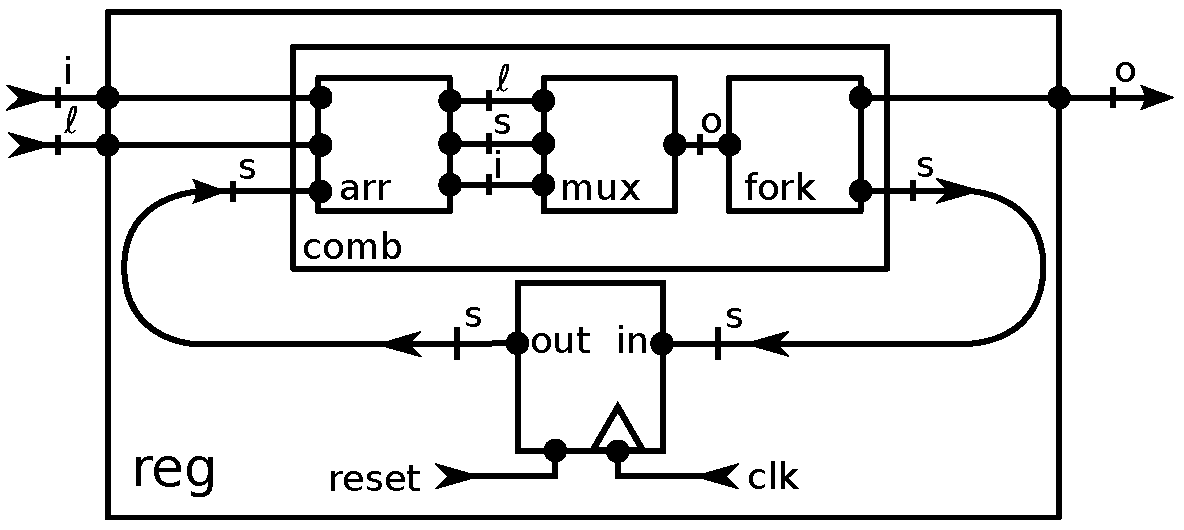
\includegraphics[width=1.0\textwidth]{imgs/register.pdf}
                \caption{Block diagram for the register described in Listing~\ref{lst:reg}.
                    \label{fig:reg}}
            \end{figure}

            The first input is the bit effectively being read and stored; this input is named "\texttt{i}".
            The second input is a control bit, telling whether or not the first input should be "loaded"
            into the register state; its name is therefore "ℓ" (for \emph{load}).
            The register's output pin simply exposes the register's internal state at any point in time.

            Also, this circuit has both an \emph{asynchronous reset} and \emph{clock} inputs,
            which are present in the synthesized netlist but \emph{not} in the Π-Ware model.
            This, in fact, applies to all sequential circuits: they all result in netlist with two extra
            inputs (\emph{reset} and \emph{clock}) which cannot be observed through an Agda interface.

            The Π-Ware code for this circuit (\AF{reg}) is shown in Listing~\ref{lst:reg}.

            \begin{listing}[h]
                \centering{\ExecuteMetaData[code/agda/latex/PiWare/Samples/BoolTrioSeq.tex]{reg}}
                \caption{Sample register circuit description.\label{lst:reg}}
            \end{listing}

            The way in which \AF{reg} is defined matches precisely the block diagram: \AF{delayℂ}
            introduces the loopback and the flip-flop "around" the combinational subcircuit (\AF{comb}).
            This combinational subcircuit consist mainly of a \emph{multiplexer},
            "choosing" whether to use the current state or current input as next state.
            Lastly, this multiplexer is wrapped by some \AI{Plug}s that serve only to change the
            ordering of some wires, performing no computation at all.

            The behaviour of this circuit is such that, with the "load" ping high, it will output
            its current input \emph{and} set the state of the flip-flop.
            With the "load" ping low, the output in clock cycle $n+1$ is equal to the input value
            in clock cycle $n$. One example of this behaviour is shown below:

            \begin{center}
                \ExecuteMetaData[code/agda/latex/PiWare/ProofSamples/BoolTrioSeq.tex]{load2}
            \end{center}

            In this example, the "load" pin is high for two clock cycles, and afterwards remains forever low.
            We are "sampling" seven elements from the register's (infinite) output \AD{Stream} and comparing
            them to an \emph{expected} vector on the right-hand side of the equality (\AF{\_≡\_}).
            We also renamed the vector prepending operator (\emph{cons}) to \AI{\_◁\_}, in order
            to avoid confusion with the \AD{Stream} prepending operator (\AI{\_∷\_}).
            Notice how the register output is "imitating" the input, because during the first two
            clock cycles the "load" pin is kept high. After that, a change in input will not cause a
            change in output.

            Naturally, we would like to prove these sorts of properties about sequential circuits
            for \emph{infinite} input and output streams.
            We would like to proof, for example, that if the "load" pin is lowered and kept low
            \emph{forever}, then the output value will \emph{never} change anymore.
            However, proofs involving coinductive types in general (and \AD{Stream}s in specific)
            are harder than regular proofs in Agda.

            The first difficulty is related to a notion of \emph{equality} between \AD{Stream}s.
            Usually, equality proofs in Agda use \emph{propositional equality}, defined as a
            datatype (\AD{\_≡\_}) in Agda's standard library (\AM{Relation.Binary.PropositionalEquality}).
            It boils down to the fact that two terms are considered equal \emph{if and only if}
            they have identical (syntactically speaking) \emph{normal forms}.

            But then, terms constructed by coinduction do not \emph{normalize} as usual.
            Terms which intuitively we would expect to be equal have \emph{suspension points}
            and will not compare equal according to \emph{propositional equality}.
            The proper notion of "sameness" for infinite \AD{Stream}s is that of \emph{bisimilarity}:
            two \AD{Stream}s are said to be \emph{bisimilar if and only if}:

            \begin{itemize}
                \item Their \emph{head} is \emph{equal} − \emph{propositionally equal}
                \item Their \emph{tail} is \emph{bisimilar}
            \end{itemize}

            Thus, the proof of bisimilarity can also be seen as a \emph{stream of equality proofs},
            one for each position in the \AD{Stream}s being compared.
            The definition of \AD{\_≈\_} is contained in Agda's standard library (\AM{Data.Stream}),
            and reproduced here for convenience:

            \begin{center}
                \ExecuteMetaData[code/agda/latex/Report/ChapterPiWare.tex]{bisimilarity}
            \end{center}

            Due to these difficulties with bisimilarity we do not currently have a proof of correctness
            for the sequential behaviour of \AF{reg}.
            We also believe that this difficulty is somewhat related to the way in which the
            \emph{causal step semantics} is converted into a \emph{stream semantics} by the
            \AF{runc} function, described in Listing~\ref{lst:run-causal}.

            Unfortunately, these investigations will have to remain for future work.
            However, we expect to be able to attack this issue by developing more general
            \emph{proof combinators} for both combinational and sequential circuits.

